\section{Pianificazione}
\groupName\:ha deciso di suddividere la pianificazione di progetto in tre fasi:
\begin{itemize}
    \item Analisi;
    \item Progettazione di dettaglio e codifica;
    \item Validazione e collaudo.
\end{itemize}

\subsection{Analisi}
Periodo: dal \textbf{2022/11/04} al \textbf{2023/02/08} \newline
Questo periodo ha inizio con l'assegnazione del capitolato d'appalto e termina con l'inizio del periodo di \textit{Proof of Concept}\glo.
Prima di tutto vengono definiti gli strumenti per la comunicazione del gruppo e gli strumenti da utilizzare per il lavoro collaborativo e
per la redazione dei documenti. Successivamente si analizza il capitolato per individuare i requisiti fondamentali, comunicando anche con
il proponente.
Inoltre si è deciso di svolgere una fase di autoformazione per studiare ed apprendere le nuove tecnologie da utilizzare per lo sviluppo del prodotto.
Le attività di questo periodo sono:
\begin{itemize}
    \item \textbf{Autoformazione}: i membri del gruppo si impegnano ad apprendere le nuove tecnologie scelte;
    \item \textbf{Analisi dei requisiti}: l'\roleAnalyst, attraverso lo studio del capitolato e la comunicazione con il proponente,
          individua i requisiti iniziali del prodotto e ne ricava le funzioni principali. Le funzioni sono rappresentate nel documento
          con l'ausilio di diagrammi UML\glo . I requisiti potrebbero evolvere nel tempo in base ai feedback del proponente;
    \item \textbf{Norme di progetto}: in questo documento vengono sono decisi gli strumenti da utilizzare nello sviluppo del prodotto
          e le regole a cui il team dovrà attenersi per la stesura di tutti i documenti. L'\roleAdministrator\:ha il compito di emanare
          le norme;
    \item \textbf{Piano di progetto}: il \roleProjectManager\:illustra un prospetto di pianificazione dettagliata, con attività e compiti,
          a cui il gruppo dovrà attenersi;
    \item \textbf{Piano di qualifica}: il documento ha lo scopo di decidere le procedura per la verifica della qualità e
          offre una visione sull'esito delle verifiche sul prodotto e i suoi componenti;
    \item \textbf{Glossario}: al fine di garantire chiarezza ed evitare ambiguità, viene redatto un glossario contenente tutti i termini necessari di definizione.
\end{itemize}
\subsubsection{\rom{1} Periodo}
Dal \textbf{2022/11/14} al \textbf{2022/11/19}
\newline
Nei primi giorni dell'analisi si discutono le norme per il lavoro collaborativo e si decidono i primi strumenti da utilizzare per
la stesura e la condivisione della documentazione relativa al prodotto. Inoltre si redigono i primi verbali relativi agli incontri
del gruppo.

\subsubsection{\rom{2} Periodo}
Dal \textbf{2022/11/20} al \textbf{2023/01/28}
\newline
In questo periodo viene redatta la documentazione del prodotto. Il gruppo decide di tenere degli incontri settimanali per discutere di
eventuali problemi riscontrati e per verificare i progressi fatti. La comunicazione con il proponente avviene tramite un canale
\textit{Discord}\glo\:dedicato.

\subsubsection{\rom{3} Periodo}
Dal \textbf{2023/01/29} al \textbf{2023/02/05}
\newline
Nell'ultimo periodo di analisi viene verificata la correttezza della documentazione basandosi anche su quanto scritto
sulle \textit{Norme di progetto v1.0.0}. Viene aggiornato il \textit{Glossario v1.0.0} con gli ultimi termini.

\begin{figure}[H]
    \centering
    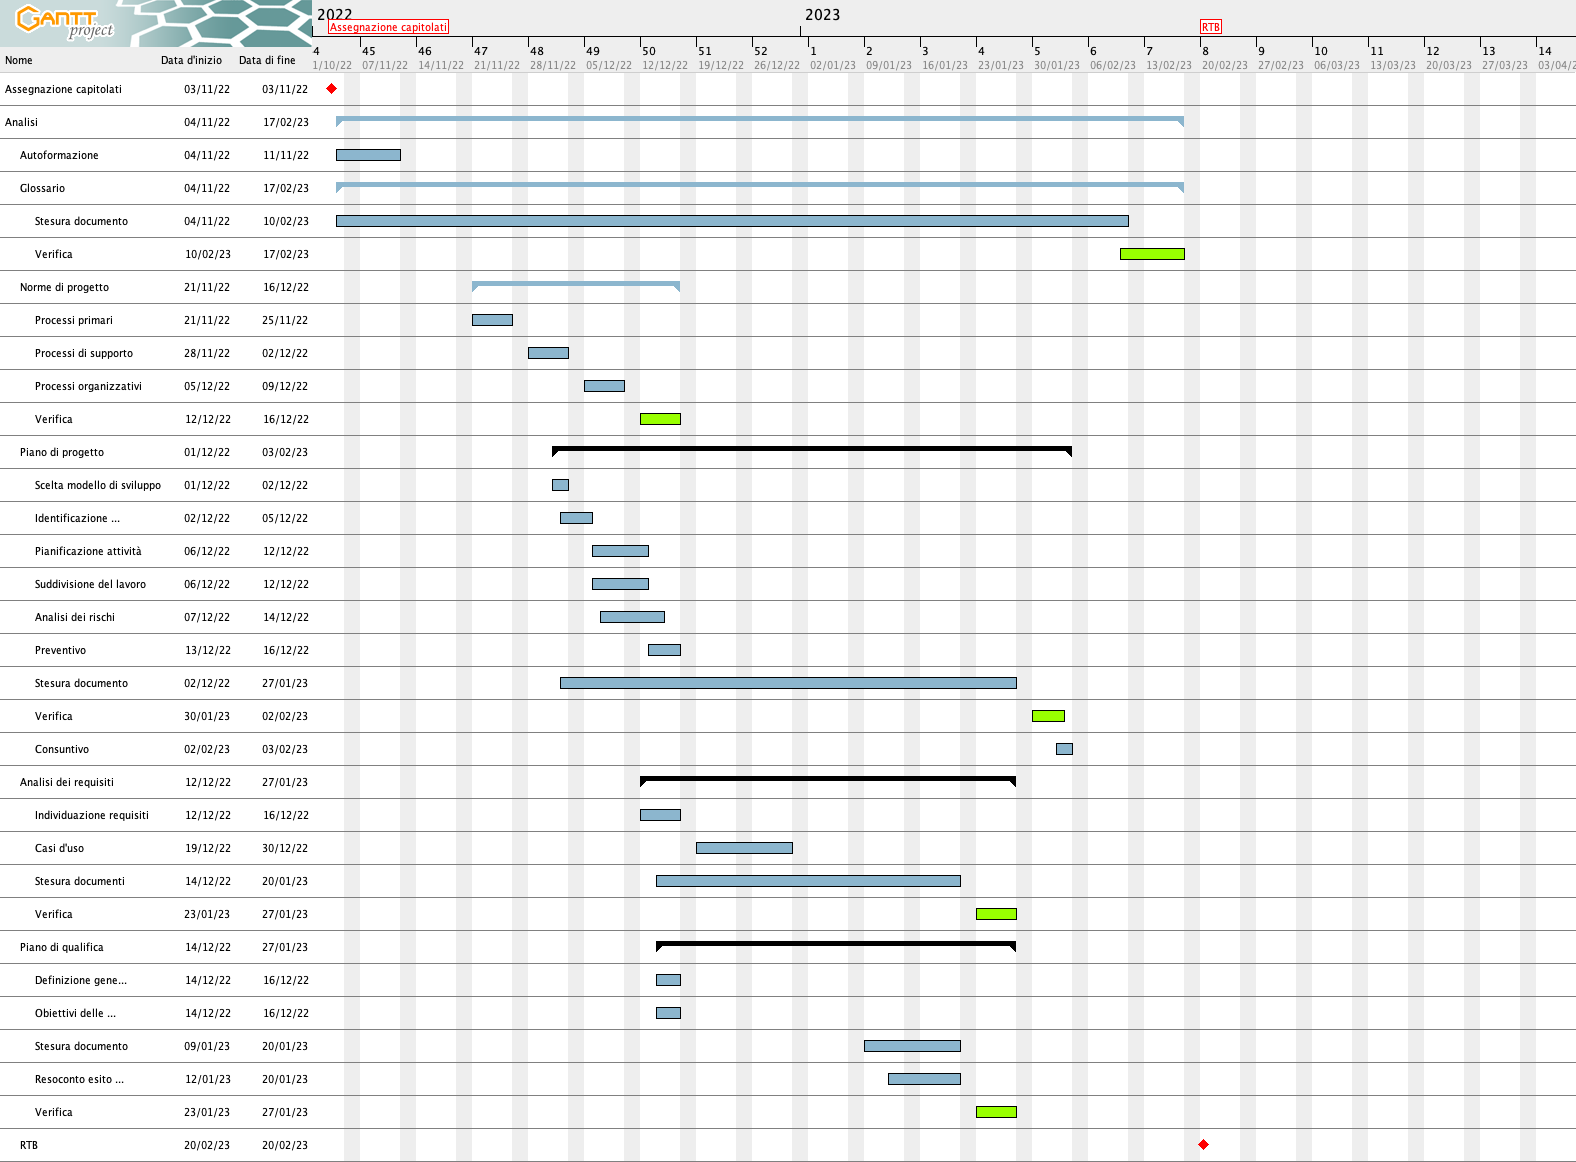
\includegraphics[scale=0.3]{src/img/Gantt analisi.png}
    \caption{Diagramma di Gantt\glo\:per l'attività di analisi}
\end{figure}

\subsection{Proof of Concept}
Periodo: dal \textbf{2023/02/06} al \textbf{2023/02/20} \newline
Questo periodo inizia al termine della verifica della documentazione e la sua fine coincide con la scadenza
di consegna dei documenti per la revisione RTB\glo.
Al termine di questo periodo verrà organizzato un incontro con il proponente per presentare un prototipo del prodotto.\newline
Si hanno due attività:
\begin{itemize}
    \item \textbf{Proof of Concept}: viene realizzato un \textit{Proof of Concept} che dovrà implementare la maggior
          parte delle tecnologie necessarie e svolgerà alcune funzioni principali del prodotto. Il PoC è un dimostrabile eseguibile
          e verrà usato come base di partenza per gli incrementi futuri;
    \item \textbf{Modifiche e verifica sui documenti}: i documenti redatti durante la fase di analisi vengono aggiornati e migliorati.
\end{itemize}
\subsubsection{\rom{1} Periodo}
Dal \textbf{2023/02/06} al \textbf{2023/02/08}
\newline
Il gruppo si impegna a studiare ed apprendere il funzionamento delle tecnologie utili e necessarie per la produzione del \textit{PoC}.

\subsubsection{\rom{2} Periodo}
Dal \textbf{2023/02/09} al \textbf{2023/02/17}
\newline
Viene sviluppato il \textit{PoC} secondo le tecnologie scelte e si implementeranno le funzioni principali del prodotto.

\subsubsection{\rom{3} Periodo}
Dal \textbf{2023/02/18} al \textbf{2023/02/20}
\newline
Nell'ultimo periodo viene redatta la presentazione per la \textit{Requirements and Technology Baseline}.

\begin{figure}[H]
    \centering
    \includegraphics[scale=0.4]{src/img/Gantt PoC.png}
    \caption{Diagramma di Gantt dell'attività di \textit{PoC}}
\end{figure}

\subsection{Progettazione di dettaglio e codifica}
Periodo: dal \textbf{2023/03/20} al \textbf{2023/05/07} \newline
Questo periodo inizia solo se si è superata la \textit{Requirements and Technology Baseline}. Viene utilizzato il \textit{PoC}
come base di partenza per il prodotto. Le attività che compongono questo periodo sono:
\begin{itemize}
    \item \textbf{Product Baseline\glo }: presenta l'architettura del prodotto attraverso il diagramma delle classi;
    \item \textbf{Codifica}: i programmatori sviluppano il codice delle funzionalità del prodotto, aggiornando e migliorando quello già presente nel \textit{PoC};
    \item \textbf{Test}: vengono sviluppati i test di unità;
    \item \textbf{Manuali}: Redazione del \textit{Manuale utente} e del \textit{Manuale sviluppatore} per l'utilizzo del prodotto;
    \item \textbf{Modifiche ai documenti}: i documenti redatti durante le fasi precedenti vengono aggiornati e migliorati.
\end{itemize}

\subsubsection{\rom{1} Sprint}
Dal \textbf{2023/03/20} al \textbf{2023/03/26}
\newline
Gli obiettivi che il gruppo si prepone per questo sprint sono:
\begin{itemize}
    \item Correzione della documentazione in base alle segnalazioni ricevute;
    \item Impostazioni delle attività di progettazione e codifica di dettaglio.
\end{itemize}
Le attività svolte sono:
\begin{itemize}
    \item Correzione della documentazione in base alle segnalazioni ricevute;
    \item Impostazioni delle attività di progettazione e codifica di dettaglio.
\end{itemize}
\begin{figure}[H]
    \centering
    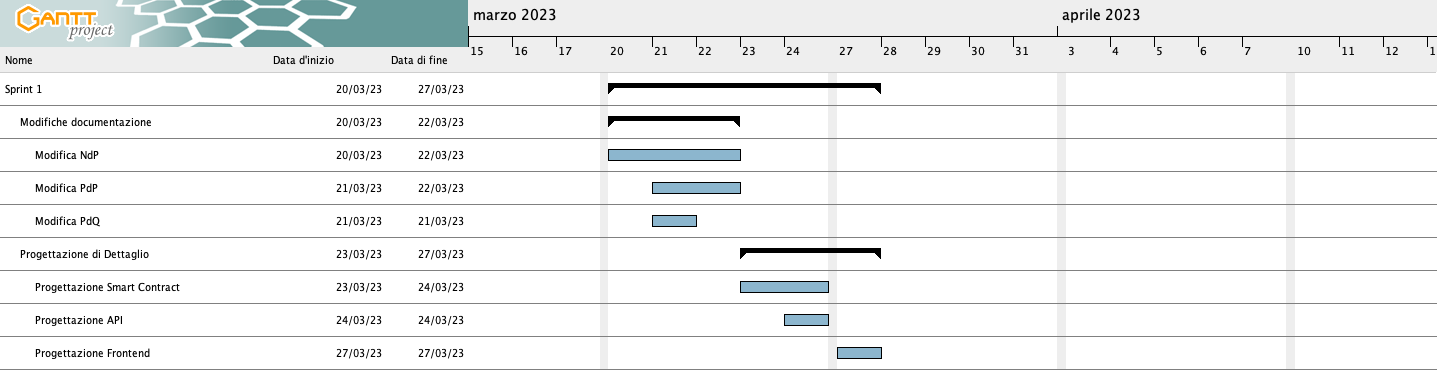
\includegraphics[scale=0.32]{src/img/GanttSprint1.png}
    \caption{Diagramma di Gantt: per il primo sprint}
\end{figure}
\subsubsection{\rom{2} Sprint}
Dal \textbf{2023/03/27} al \textbf{2023/04/02}
\newline
Dopo un incontro con l'azienda committente sono stati chiariti alcuni dubbi sorti durante le riunioni tra i membri del gruppo.
\newline
Gli obiettivi che il gruppo si prepone per questo sprint sono:
\begin{itemize}
    \item Studio approfondito di tutte le tecnologie in uso;
    \item Inizio progettazione di dettaglio con principali classi;
    \item Continuazione stesura documentazione.
\end{itemize}
Le attività svolte sono:
\begin{itemize}
    \item Documentazione: aggiornamento \textit{AdR, PdP, Pdq};
    \item Progettazione: Smart contract, API e frontend;
    \item Apprendimento nuove funzionalità.

\end{itemize}
\begin{figure}[H]
    \centering
    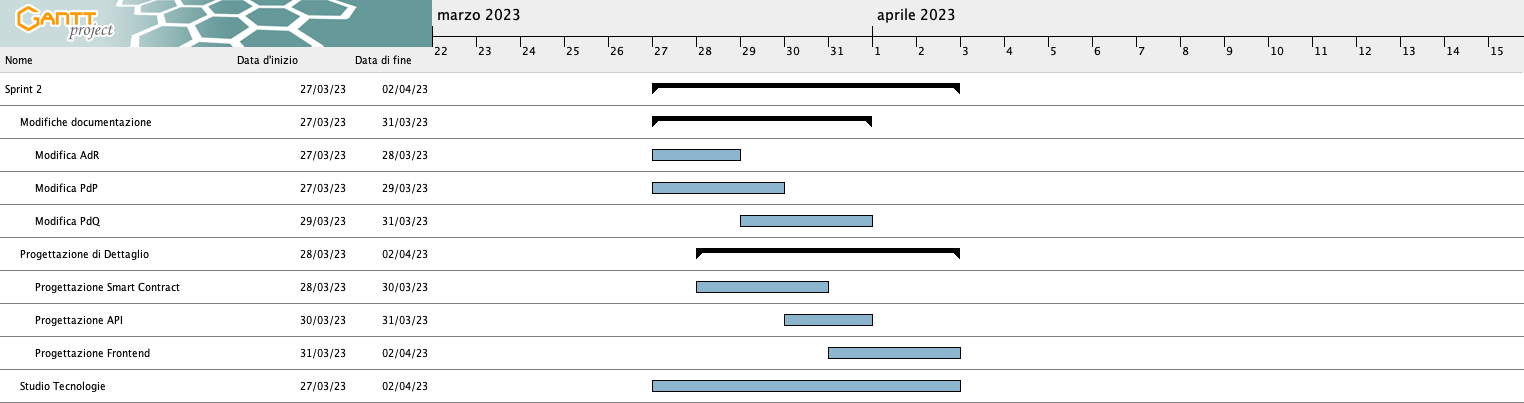
\includegraphics[scale=0.32]{src/img/Sprint 2.png}
    \caption{Diagramma di Gantt: per il secondo sprint}
\end{figure}
\subsubsection{\rom{3} Sprint}
Dal \textbf{2023/04/03} al \textbf{2023/04/09}
\newline
Gli obiettivi che il gruppo si prepone per questo sprint sono:
\begin{itemize}
    \item Refactoring dello smart contract;
    \item Continuazione stesura della documentazione da correlare al prodotto software.
\end{itemize}
Le attività svolte sono:
\begin{itemize}
    \item Documentazione: aggiornamento \textit{NdP, PdP, Pdq};
    \item Sviluppo: struttura principale smart contract.
\end{itemize}
\begin{figure}[H]
    \centering
    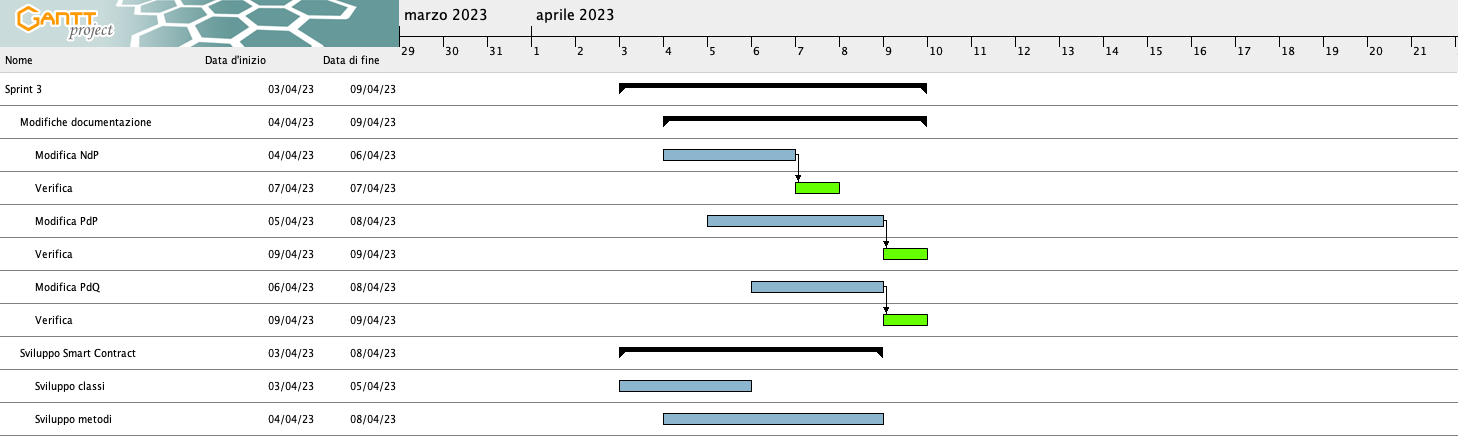
\includegraphics[scale=0.32]{src/img/Sprint 3.png}
    \caption{Diagramma di Gantt: per il terzo sprint}
\end{figure}
\subsubsection{\rom{4} Sprint}
Dal \textbf{2023/04/10} al \textbf{2023/04/16}
\newline
Gli obiettivi che il gruppo si prepone per questo sprint sono:
\begin{itemize}
    \item Inizio refactoring del frontend associato;
    \item Stesura test di unità;
    \item Continuazione stesura della documentazione da correlare al prodotto software;
\end{itemize}
Le attività svolte sono:
\begin{itemize}
    \item Documentazione: aggiornamento \textit{PdP, Pdq};
    \item Sviluppo: ampliamento frontend del PoC.
\end{itemize}
\begin{figure}[H]
    \centering
    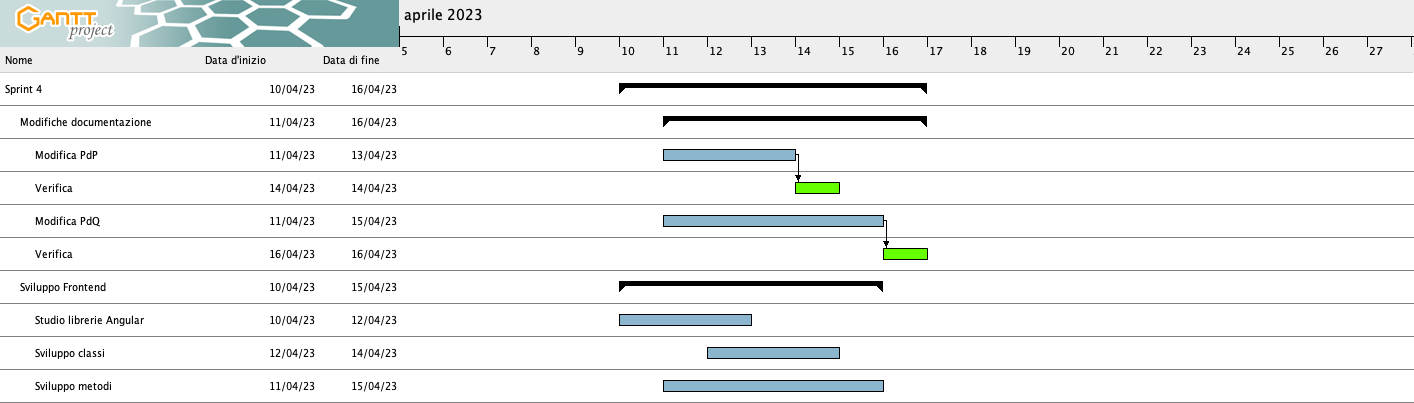
\includegraphics[scale=0.32]{src/img/Sprint 4.png}
    \caption{Diagramma di Gantt: per il quarto sprint}
\end{figure}
\subsubsection{\rom{5} Sprint}
Dal \textbf{2023/04/17} al \textbf{2023/04/23}
\newline
Gli obiettivi che il gruppo si prepone per questo sprint sono:
\begin{itemize}
    \item Stesura \textit{Specifica Tecnica};
    \item Continuazione implementazione frontend;
    \item Continuazione stesura della documentazione da correlare al prodotto software.
\end{itemize}
Le attività svolte sono:
\begin{itemize}
    \item Documentazione: stesura \textit{Specifica Tecnica} e aggiornamento \textit{PdP, Pdq};
    \item Sviluppo: integrazione del frontend con smart contract e API.
\end{itemize}
\begin{figure}[H]
    \centering
    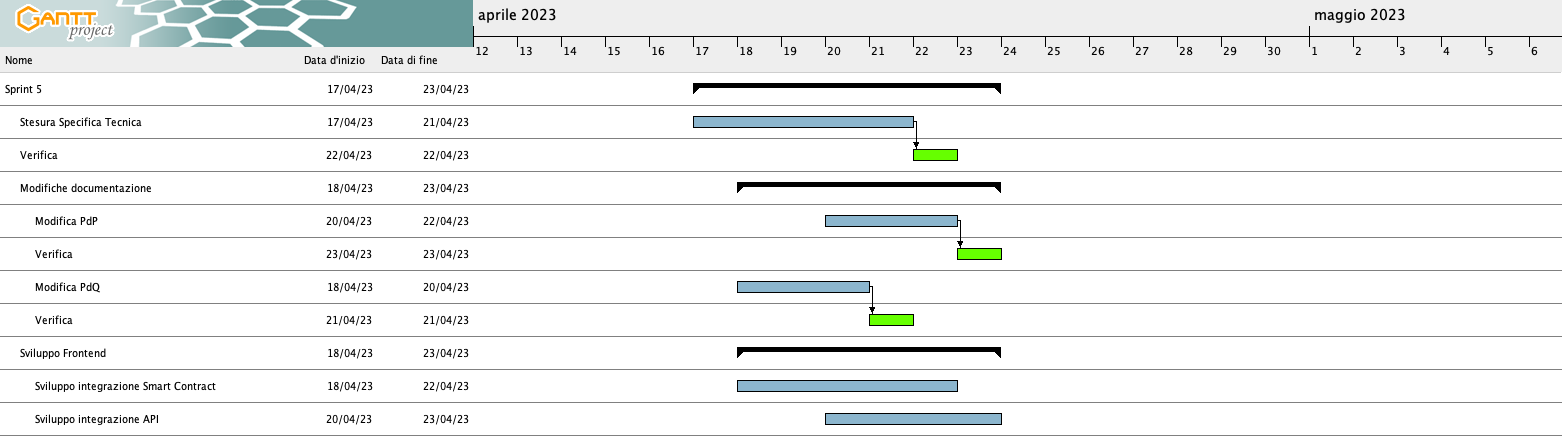
\includegraphics[scale=0.32]{src/img/Sprint 5.png}
    \caption{Diagramma di Gantt: per il quinto sprint}
\end{figure}
\subsubsection{\rom{6} Sprint}
Dal \textbf{2023/04/24} al \textbf{2023/04/30}
\newline
Gli obiettivi che il gruppo si prepone per questo sprint sono:
\begin{itemize}
    \item Revisione e avanzamento progettazione;
    \item Conclusione smart contract;
    \item Sviluppo e conclusione API;
    \item Stesura \textit{Manuale Utente};
    \item Continuazione stesura della documentazione da correlare al prodotto software.
\end{itemize}
Le attività svolte sono:
\begin{itemize}
    \item Documentazione: stesura \textit{Manuale Utente} e aggiornamento \textit{AdR, ST, Pdq};
    \item Sviluppo: continuazione sviluppo smart contract e API;
    \item Progettazione: correzione di alcuni elementi della progettazione già reallizzata.
\end{itemize}
\begin{figure}[H]
    \centering
    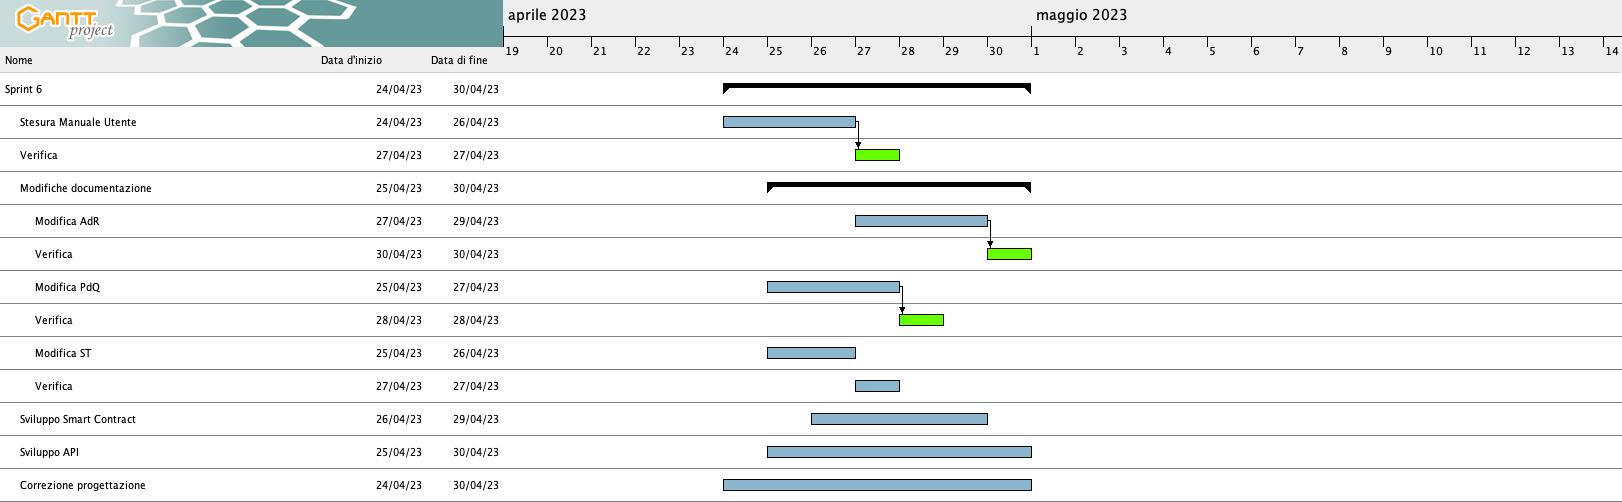
\includegraphics[scale=0.32]{src/img/Sprint 6.png}
    \caption{Diagramma di Gantt: per il sesto sprint}
\end{figure}
\subsubsection{\rom{7} Sprint}
Dal \textbf{2023/05/01} al \textbf{2023/05/07}
\newline
Gli obiettivi che il gruppo si prepone per questo sprint sono:
\begin{itemize}
    \item Verifica finale dei test
    \item Conclusione stesura della documentazione da correlare al prodotto software.
\end{itemize}
Le attività svolte sono:
\begin{itemize}
    \item Documentazione: aggiornamento e verifica finale di tutti i documenti prodotti;
    \item Test: esecuzione di tutti i test stabiliti.
\end{itemize}
\begin{figure}[H]
    \centering
    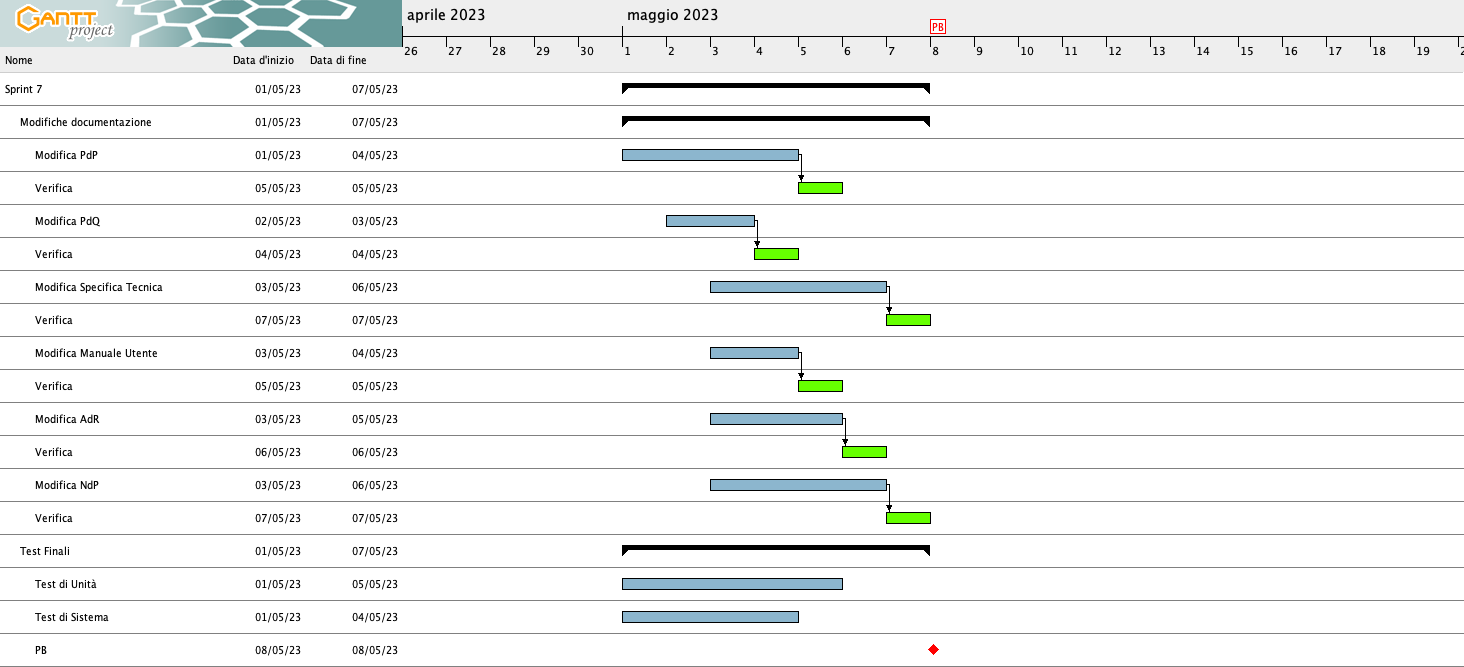
\includegraphics[scale=0.32]{src/img/Sprint 7.png}
    \caption{Diagramma di Gantt: per il settimo sprint}
\end{figure}

% \subsection{VALIDAZIONE???}

\section{Preventivo dei costi}
\subsection{Analisi}
\subsubsection{Prospetto orario}
\rowcolors{2}{pari_alt}{dispari_alt}
\renewcommand{\arraystretch}{1.8}

\begin{xltabular}{\textwidth} {
        >{\hsize=1.70\hsize\linewidth=\hsize}X
        >{\hsize=0.5\hsize\linewidth=\hsize}X
        >{\hsize=0.5\hsize\linewidth=\hsize}X
        >{\hsize=0.5\hsize\linewidth=\hsize}X
        >{\hsize=0.5\hsize\linewidth=\hsize}X
        >{\hsize=0.5\hsize\linewidth=\hsize}X
        >{\hsize=0.5\hsize\linewidth=\hsize}X
        >{\hsize=0.8\hsize\linewidth=\hsize}X
    }
    \rowcolorhead
    \textbf{\color{white}Componente} &
    \textbf{\color{white}Re} &
    \textbf{\color{white}Pt} &
    \textbf{\color{white}An} &
    \textbf{\color{white}Am} &
    \textbf{\color{white}Pr} &
    \textbf{\color{white}Ve} &
    \textbf{\color{white}Totale} \\
    \hline
    \endfirsthead

    \hline
    \rowcolorhead
    \textbf{\color{white}Componente} &
    \textbf{\color{white}Re} &
    \textbf{\color{white}Pt} &
    \textbf{\color{white}An} &
    \textbf{\color{white}Am} &
    \textbf{\color{white}Pr} &
    \textbf{\color{white}Ve} &
    \textbf{\color{white}Totale} \\
    \hline
    \endhead

    \endfoot

    \endlastfoot

    Elia Pasquali & 4 & 0 & 11 & 7 & 0 & 6 & 28 \\
    Ennio Italiano & 4 & 0 & 13 & 6 & 0 & 7 & 30 \\
    Enrico Bacci Bonivento & 4 & 0 & 11 & 6 & 0 & 7 & 28 \\
    Fabio Pantaleo & 4 & 0 & 11 & 6 & 0 & 7 & 28 \\
    Nicolò Trinca & 4 & 0 & 12 & 7 & 0 & 6 & 29 \\
    Sebastiano Sanson & 6 & 0 & 12 & 7 & 0 & 6 & 31 \\
    Totale & 26 & 0 & 70 & 39 & 0 & 39 & 174\\
    % & & & & & & &
    \rowcolor{white}
    \caption{Distribuzione delle ore nel periodo di analisi}
\end{xltabular}

\subsubsection{Prospetto economico}
\rowcolors{2}{pari_alt}{dispari_alt}
\renewcommand{\arraystretch}{1.8}

\begin{xltabular}{\textwidth} {
        >{\hsize=1\hsize\linewidth=\hsize}X
        >{\hsize=0.5\hsize\linewidth=\hsize}X
        >{\hsize=0.5\hsize\linewidth=\hsize}X
    }
    \rowcolorhead
    \textbf{\color{white}Ruolo} &
    \textbf{\color{white}Totale ore} &
    \textbf{\color{white}Costo totale} \\
    \hline
    \endfirsthead

    \hline
    \rowcolorhead
    \textbf{\color{white}Ruolo} &
    \textbf{\color{white}Totale ore} &
    \textbf{\color{white}Costo totale} \\
    \hline
    \endhead

    \endfoot

    \endlastfoot

    Responsabile & 26 & 780 \\
    Progettista & 0 & 0 \\
    Analista & 70 & 1750\\
    Amministratore & 39 & 780 \\
    Programmatore & 0 & 0  \\
    Verificatore & 39 & 585 \\
    Totale & 174 & 3895 \\
    % & & & & & & &
    \rowcolor{white}
    \caption{Prospetto dei costi per ruolo nel periodo di analisi}
\end{xltabular}

\subsection{Proof of Concept}
\subsubsection{Prospetto orario}
\rowcolors{2}{pari_alt}{dispari_alt}
\renewcommand{\arraystretch}{1.8}

\begin{xltabular}{\textwidth} {
        >{\hsize=1.70\hsize\linewidth=\hsize}X
        >{\hsize=0.5\hsize\linewidth=\hsize}X
        >{\hsize=0.5\hsize\linewidth=\hsize}X
        >{\hsize=0.5\hsize\linewidth=\hsize}X
        >{\hsize=0.5\hsize\linewidth=\hsize}X
        >{\hsize=0.5\hsize\linewidth=\hsize}X
        >{\hsize=0.5\hsize\linewidth=\hsize}X
        >{\hsize=0.8\hsize\linewidth=\hsize}X
    }
    \rowcolorhead
    \textbf{\color{white}Componente} &
    \textbf{\color{white}Re} &
    \textbf{\color{white}Pt} &
    \textbf{\color{white}An} &
    \textbf{\color{white}Am} &
    \textbf{\color{white}Pr} &
    \textbf{\color{white}Ve} &
    \textbf{\color{white}Totale} \\
    \hline
    \endfirsthead

    \hline
    \rowcolorhead
    \textbf{\color{white}Componente} &
    \textbf{\color{white}Re} &
    \textbf{\color{white}Pt} &
    \textbf{\color{white}An} &
    \textbf{\color{white}Am} &
    \textbf{\color{white}Pr} &
    \textbf{\color{white}Ve} &
    \textbf{\color{white}Totale} \\
    \hline
    \endhead

    \endfoot

    \endlastfoot

    Elia Pasquali & 2 & 4 & 2 & 5 & 5 & 2 & 20 \\
    Ennio Italiano & 1 & 4 & 2 & 6 & 6 & 2 & 21 \\
    Enrico Bacci Bonivento & 2 & 5 & 1 & 4 & 6 & 2 & 20 \\
    Fabio Pantaleo & 1 & 6 & 1 & 2 & 7 & 2 & 19 \\
    Nicolò Trinca & 1 & 5 & 0 & 3 & 8 & 2 & 19 \\
    Sebastiano Sanson & 2 & 6 & 0 & 3 & 6 & 2 & 19 \\
    Totale & 9 & 30 & 6 & 23 & 38 & 12 & 118 \\
    % & & & & & & &
    \rowcolor{white}
    \caption{Distribuzione delle ore nel periodo di \textit{Proof of Concept}}
\end{xltabular}

\subsubsection{Prospetto economico}
\rowcolors{2}{pari_alt}{dispari_alt}
\renewcommand{\arraystretch}{1.8}

\begin{xltabular}{\textwidth} {
        >{\hsize=1\hsize\linewidth=\hsize}X
        >{\hsize=0.5\hsize\linewidth=\hsize}X
        >{\hsize=0.5\hsize\linewidth=\hsize}X
    }
    \rowcolorhead
    \textbf{\color{white}Ruolo} &
    \textbf{\color{white}Totale ore} &
    \textbf{\color{white}Costo totale} \\
    \hline
    \endfirsthead

    \hline
    \rowcolorhead
    \textbf{\color{white}Ruolo} &
    \textbf{\color{white}Totale ore} &
    \textbf{\color{white}Costo totale} \\
    \hline
    \endhead

    \endfoot

    \endlastfoot

    Responsabile & 9 & 270 \\
    Progettista & 30 & 750 \\
    Analista & 6 & 150\\
    Amministratore & 23 & 460 \\
    Programmatore & 38 & 570  \\
    Verificatore & 12 & 180 \\
    Totale & 118 & 2380 \\
    % & & & & & & &
    \rowcolor{white}
    \caption{Prospetto dei costi per ruolo nel periodo di \textit{Proof of Concept}}
\end{xltabular}

\subsection{Progettazione di dettaglio e codifica dei requisiti}
\subsubsection{Sprint 1}
\paragraph{Prospetto orario}

\rowcolors{2}{pari_alt}{dispari_alt}
\renewcommand{\arraystretch}{1.8}

\begin{xltabular}{\textwidth} {
        >{\hsize=1.70\hsize\linewidth=\hsize}X
        >{\hsize=0.5\hsize\linewidth=\hsize}X
        >{\hsize=0.5\hsize\linewidth=\hsize}X
        >{\hsize=0.5\hsize\linewidth=\hsize}X
        >{\hsize=0.5\hsize\linewidth=\hsize}X
        >{\hsize=0.5\hsize\linewidth=\hsize}X
        >{\hsize=0.5\hsize\linewidth=\hsize}X
        >{\hsize=0.8\hsize\linewidth=\hsize}X
    }
    \rowcolorhead
    \textbf{\color{white}Componente} &
    \textbf{\color{white}Re} &
    \textbf{\color{white}Pt} &
    \textbf{\color{white}An} &
    \textbf{\color{white}Am} &
    \textbf{\color{white}Pr} &
    \textbf{\color{white}Ve} &
    \textbf{\color{white}Totale} \\
    \hline
    \endfirsthead

    \hline
    \rowcolorhead
    \textbf{\color{white}Componente} &
    \textbf{\color{white}Re} &
    \textbf{\color{white}Pt} &
    \textbf{\color{white}An} &
    \textbf{\color{white}Am} &
    \textbf{\color{white}Pr} &
    \textbf{\color{white}Ve} &
    \textbf{\color{white}Totale} \\
    \hline
    \endhead

    \endfoot

    \endlastfoot

    Elia Pasquali           & 1 & 0 & 1 & 0 & 0 & 1 & 3 \\
    Ennio Italiano          & 0 & 2 & 0 & 0 & 0 & 1 & 3 \\
    Enrico Bacci Bonivento  & 0 & 1 & 0 & 0 & 1 & 1 & 3 \\
    Fabio Pantaleo          & 1 & 1 & 0 & 0 & 0 & 1 & 3 \\
    Nicolò Trinca           & 0 & 1 & 0 & 0 & 1 & 0 & 2 \\
    Sebastiano Sanson       & 0 & 1 & 1 & 1 & 0 & 0 & 3 \\
    Totale                  & 2 & 6 & 2 & 1 & 2 & 4 & 17 \\
    % & & & & & & &
    \rowcolor{white}
    \caption{Distribuzione delle ore nel primo sprint}
\end{xltabular}

\paragraph{Prospetto economico}
\rowcolors{2}{pari_alt}{dispari_alt}
\renewcommand{\arraystretch}{1.8}

\begin{xltabular}{\textwidth} {
        >{\hsize=1\hsize\linewidth=\hsize}X
        >{\hsize=0.5\hsize\linewidth=\hsize}X
        >{\hsize=0.5\hsize\linewidth=\hsize}X
    }
    \rowcolorhead
    \textbf{\color{white}Ruolo} &
    \textbf{\color{white}Totale ore} &
    \textbf{\color{white}Costo totale} \\
    \hline
    \endfirsthead

    \hline
    \rowcolorhead
    \textbf{\color{white}Ruolo} &
    \textbf{\color{white}Totale ore} &
    \textbf{\color{white}Costo totale} \\
    \hline
    \endhead

    \endfoot

    \endlastfoot

    Responsabile & 2 & 60 \\
    Progettista & 6 & 150 \\
    Analista & 2 & 50 \\
    Amministratore & 1 & 20 \\
    Programmatore & 2 & 30  \\
    Verificatore & 4 & 60 \\
    Totale & 17 & 370 \\
    % & & & & & & &
    \rowcolor{white}
    \caption{Prospetto dei costi per ruolo nel primo sprint}
\end{xltabular}
\subsubsection{Sprint 2}
\paragraph{Prospetto orario}

\rowcolors{2}{pari_alt}{dispari_alt}
\renewcommand{\arraystretch}{1.8}

\begin{xltabular}{\textwidth} {
        >{\hsize=1.70\hsize\linewidth=\hsize}X
        >{\hsize=0.5\hsize\linewidth=\hsize}X
        >{\hsize=0.5\hsize\linewidth=\hsize}X
        >{\hsize=0.5\hsize\linewidth=\hsize}X
        >{\hsize=0.5\hsize\linewidth=\hsize}X
        >{\hsize=0.5\hsize\linewidth=\hsize}X
        >{\hsize=0.5\hsize\linewidth=\hsize}X
        >{\hsize=0.8\hsize\linewidth=\hsize}X
    }
    \rowcolorhead
    \textbf{\color{white}Componente} &
    \textbf{\color{white}Re} &
    \textbf{\color{white}Pt} &
    \textbf{\color{white}An} &
    \textbf{\color{white}Am} &
    \textbf{\color{white}Pr} &
    \textbf{\color{white}Ve} &
    \textbf{\color{white}Totale} \\
    \hline
    \endfirsthead

    \hline
    \rowcolorhead
    \textbf{\color{white}Componente} &
    \textbf{\color{white}Re} &
    \textbf{\color{white}Pt} &
    \textbf{\color{white}An} &
    \textbf{\color{white}Am} &
    \textbf{\color{white}Pr} &
    \textbf{\color{white}Ve} &
    \textbf{\color{white}Totale} \\
    \hline
    \endhead

    \endfoot

    \endlastfoot

    Elia Pasquali           & 0 & 5 & 1 & 0 & 0 & 0 & 6 \\
    Ennio Italiano          & 1 & 3 & 0 & 0 & 0 & 0 & 4 \\
    Enrico Bacci Bonivento  & 1 & 3 & 0 & 0 & 0 & 0 & 4 \\
    Fabio Pantaleo          & 0 & 4 & 0 & 0 & 1 & 0 & 5 \\
    Nicolò Trinca           & 0 & 4 & 0 & 1 & 0 & 0 & 5 \\
    Sebastiano Sanson       & 0 & 4 & 1 & 0 & 0 & 0 & 5 \\
    Totale                  & 2 & 23 & 2 & 1 & 1 & 0 & 29 \\
    % & & & & & & &
    \rowcolor{white}
    \caption{Distribuzione delle ore nel secondo sprint}
\end{xltabular}

\paragraph{Prospetto economico}
\rowcolors{2}{pari_alt}{dispari_alt}
\renewcommand{\arraystretch}{1.8}

\begin{xltabular}{\textwidth} {
        >{\hsize=1\hsize\linewidth=\hsize}X
        >{\hsize=0.5\hsize\linewidth=\hsize}X
        >{\hsize=0.5\hsize\linewidth=\hsize}X
    }
    \rowcolorhead
    \textbf{\color{white}Ruolo} &
    \textbf{\color{white}Totale ore} &
    \textbf{\color{white}Costo totale} \\
    \hline
    \endfirsthead

    \hline
    \rowcolorhead
    \textbf{\color{white}Ruolo} &
    \textbf{\color{white}Totale ore} &
    \textbf{\color{white}Costo totale} \\
    \hline
    \endhead

    \endfoot

    \endlastfoot

    Responsabile & 2 & 60 \\
    Progettista & 23 & 575 \\
    Analista & 2 & 50 \\
    Amministratore & 1 & 20 \\
    Programmatore & 1 & 15  \\
    Verificatore & 0 & 0 \\
    Totale & 29 & 670 \\
    % & & & & & & &
    \rowcolor{white}
    \caption{Prospetto dei costi per ruolo nel secondo sprint}
\end{xltabular}
\subsubsection{Sprint 3}
\paragraph{Prospetto orario}

\rowcolors{2}{pari_alt}{dispari_alt}
\renewcommand{\arraystretch}{1.8}

\begin{xltabular}{\textwidth} {
        >{\hsize=1.70\hsize\linewidth=\hsize}X
        >{\hsize=0.5\hsize\linewidth=\hsize}X
        >{\hsize=0.5\hsize\linewidth=\hsize}X
        >{\hsize=0.5\hsize\linewidth=\hsize}X
        >{\hsize=0.5\hsize\linewidth=\hsize}X
        >{\hsize=0.5\hsize\linewidth=\hsize}X
        >{\hsize=0.5\hsize\linewidth=\hsize}X
        >{\hsize=0.8\hsize\linewidth=\hsize}X
    }
    \rowcolorhead
    \textbf{\color{white}Componente} &
    \textbf{\color{white}Re} &
    \textbf{\color{white}Pt} &
    \textbf{\color{white}An} &
    \textbf{\color{white}Am} &
    \textbf{\color{white}Pr} &
    \textbf{\color{white}Ve} &
    \textbf{\color{white}Totale} \\
    \hline
    \endfirsthead

    \hline
    \rowcolorhead
    \textbf{\color{white}Componente} &
    \textbf{\color{white}Re} &
    \textbf{\color{white}Pt} &
    \textbf{\color{white}An} &
    \textbf{\color{white}Am} &
    \textbf{\color{white}Pr} &
    \textbf{\color{white}Ve} &
    \textbf{\color{white}Totale} \\
    \hline
    \endhead

    \endfoot

    \endlastfoot

    Elia Pasquali           & 0 & 3 & 0 & 0 & 4 & 0 & 7 \\
    Ennio Italiano          & 0 & 3 & 0 & 0 & 3 & 2 & 8 \\
    Enrico Bacci Bonivento  & 0 & 3 & 1 & 0 & 3 & 0 & 7 \\
    Fabio Pantaleo          & 0 & 3 & 0 & 1 & 4 & 0 & 8 \\
    Nicolò Trinca           & 1 & 2 & 0 & 0 & 4 & 2 & 9 \\
    Sebastiano Sanson       & 1 & 2 & 0 & 1 & 5 & 0 & 9 \\
    Totale                  & 2 & 16 & 1 & 2 & 23 & 4 & 48 \\
    % & & & & & & &
    \rowcolor{white}
    \caption{Distribuzione delle ore nel terzo sprint}
\end{xltabular}

\paragraph{Prospetto economico}
\rowcolors{2}{pari_alt}{dispari_alt}
\renewcommand{\arraystretch}{1.8}

\begin{xltabular}{\textwidth} {
        >{\hsize=1\hsize\linewidth=\hsize}X
        >{\hsize=0.5\hsize\linewidth=\hsize}X
        >{\hsize=0.5\hsize\linewidth=\hsize}X
    }
    \rowcolorhead
    \textbf{\color{white}Ruolo} &
    \textbf{\color{white}Totale ore} &
    \textbf{\color{white}Costo totale} \\
    \hline
    \endfirsthead

    \hline
    \rowcolorhead
    \textbf{\color{white}Ruolo} &
    \textbf{\color{white}Totale ore} &
    \textbf{\color{white}Costo totale} \\
    \hline
    \endhead

    \endfoot

    \endlastfoot

    Responsabile & 2 & 60 \\
    Progettista & 16 & 400 \\
    Analista & 1 & 25 \\
    Amministratore & 2 & 40 \\
    Programmatore & 23 & 345  \\
    Verificatore & 4 & 60 \\
    Totale & 48 & 930 \\
    % & & & & & & &
    \rowcolor{white}
    \caption{Prospetto dei costi per ruolo nel terzo sprint}
\end{xltabular}
\subsubsection{Sprint 4}
\paragraph{Prospetto orario}

\rowcolors{2}{pari_alt}{dispari_alt}
\renewcommand{\arraystretch}{1.8}

\begin{xltabular}{\textwidth} {
        >{\hsize=1.70\hsize\linewidth=\hsize}X
        >{\hsize=0.5\hsize\linewidth=\hsize}X
        >{\hsize=0.5\hsize\linewidth=\hsize}X
        >{\hsize=0.5\hsize\linewidth=\hsize}X
        >{\hsize=0.5\hsize\linewidth=\hsize}X
        >{\hsize=0.5\hsize\linewidth=\hsize}X
        >{\hsize=0.5\hsize\linewidth=\hsize}X
        >{\hsize=0.8\hsize\linewidth=\hsize}X
    }
    \rowcolorhead
    \textbf{\color{white}Componente} &
    \textbf{\color{white}Re} &
    \textbf{\color{white}Pt} &
    \textbf{\color{white}An} &
    \textbf{\color{white}Am} &
    \textbf{\color{white}Pr} &
    \textbf{\color{white}Ve} &
    \textbf{\color{white}Totale} \\
    \hline
    \endfirsthead

    \hline
    \rowcolorhead
    \textbf{\color{white}Componente} &
    \textbf{\color{white}Re} &
    \textbf{\color{white}Pt} &
    \textbf{\color{white}An} &
    \textbf{\color{white}Am} &
    \textbf{\color{white}Pr} &
    \textbf{\color{white}Ve} &
    \textbf{\color{white}Totale} \\
    \hline
    \endhead

    \endfoot

    \endlastfoot

    Elia Pasquali           & 0 & 3 & 0 & 0 & 4 & 0 & 7 \\
    Ennio Italiano          & 0 & 3 & 0 & 1 & 5 & 0 & 9 \\
    Enrico Bacci Bonivento  & 1 & 3 & 0 & 1 & 5 & 0 & 9 \\
    Fabio Pantaleo          & 1 & 3 & 1 & 0 & 4 & 2 & 11 \\
    Nicolò Trinca           & 0 & 4 & 0 & 0 & 4 & 0 & 8 \\
    Sebastiano Sanson       & 0 & 4 & 0 & 0 & 4 & 2 & 10 \\
    Totale                  & 2 & 20 & 1 & 2 & 26 & 4 & 55 \\
    % & & & & & & &
    \rowcolor{white}
    \caption{Distribuzione delle ore nel quarto sprint}
\end{xltabular}

\paragraph{Prospetto economico}
\rowcolors{2}{pari_alt}{dispari_alt}
\renewcommand{\arraystretch}{1.8}

\begin{xltabular}{\textwidth} {
        >{\hsize=1\hsize\linewidth=\hsize}X
        >{\hsize=0.5\hsize\linewidth=\hsize}X
        >{\hsize=0.5\hsize\linewidth=\hsize}X
    }
    \rowcolorhead
    \textbf{\color{white}Ruolo} &
    \textbf{\color{white}Totale ore} &
    \textbf{\color{white}Costo totale} \\
    \hline
    \endfirsthead

    \hline
    \rowcolorhead
    \textbf{\color{white}Ruolo} &
    \textbf{\color{white}Totale ore} &
    \textbf{\color{white}Costo totale} \\
    \hline
    \endhead

    \endfoot

    \endlastfoot

    Responsabile & 2 & 60 \\
    Progettista & 20 & 500 \\
    Analista & 1 & 25 \\
    Amministratore & 2 & 40 \\
    Programmatore & 26 & 390  \\
    Verificatore & 4 & 60 \\
    Totale & 48 & 1075 \\
    % & & & & & & &
    \rowcolor{white}
    \caption{Prospetto dei costi per ruolo nel quarto sprint}
\end{xltabular}
\subsubsection{Sprint 5}
\paragraph{Prospetto orario}

\rowcolors{2}{pari_alt}{dispari_alt}
\renewcommand{\arraystretch}{1.8}

\begin{xltabular}{\textwidth} {
        >{\hsize=1.70\hsize\linewidth=\hsize}X
        >{\hsize=0.5\hsize\linewidth=\hsize}X
        >{\hsize=0.5\hsize\linewidth=\hsize}X
        >{\hsize=0.5\hsize\linewidth=\hsize}X
        >{\hsize=0.5\hsize\linewidth=\hsize}X
        >{\hsize=0.5\hsize\linewidth=\hsize}X
        >{\hsize=0.5\hsize\linewidth=\hsize}X
        >{\hsize=0.8\hsize\linewidth=\hsize}X
    }
    \rowcolorhead
    \textbf{\color{white}Componente} &
    \textbf{\color{white}Re} &
    \textbf{\color{white}Pt} &
    \textbf{\color{white}An} &
    \textbf{\color{white}Am} &
    \textbf{\color{white}Pr} &
    \textbf{\color{white}Ve} &
    \textbf{\color{white}Totale} \\
    \hline
    \endfirsthead

    \hline
    \rowcolorhead
    \textbf{\color{white}Componente} &
    \textbf{\color{white}Re} &
    \textbf{\color{white}Pt} &
    \textbf{\color{white}An} &
    \textbf{\color{white}Am} &
    \textbf{\color{white}Pr} &
    \textbf{\color{white}Ve} &
    \textbf{\color{white}Totale} \\
    \hline
    \endhead

    \endfoot

    \endlastfoot

    Elia Pasquali           & 1 & 0 & 0 & 1 & 3 & 1 & 6 \\
    Ennio Italiano          & 1 & 0 & 0 & 0 & 3 & 1 & 5 \\
    Enrico Bacci Bonivento  & 0 & 0 & 0 & 0 & 4 & 0 & 4 \\
    Fabio Pantaleo          & 0 & 0 & 0 & 0 & 4 & 0 & 4 \\
    Nicolò Trinca           & 0 & 0 & 1 & 1 & 3 & 1 & 6 \\
    Sebastiano Sanson       & 0 & 0 & 0 & 0 & 3 & 1 & 4 \\
    Totale                  & 2 & 0 & 1 & 2 & 20 & 4 & 29 \\
    % & & & & & & &
    \rowcolor{white}
    \caption{Distribuzione delle ore nel quinto sprint}
\end{xltabular}

\paragraph{Prospetto economico}
\rowcolors{2}{pari_alt}{dispari_alt}
\renewcommand{\arraystretch}{1.8}

\begin{xltabular}{\textwidth} {
        >{\hsize=1\hsize\linewidth=\hsize}X
        >{\hsize=0.5\hsize\linewidth=\hsize}X
        >{\hsize=0.5\hsize\linewidth=\hsize}X
    }
    \rowcolorhead
    \textbf{\color{white}Ruolo} &
    \textbf{\color{white}Totale ore} &
    \textbf{\color{white}Costo totale} \\
    \hline
    \endfirsthead

    \hline
    \rowcolorhead
    \textbf{\color{white}Ruolo} &
    \textbf{\color{white}Totale ore} &
    \textbf{\color{white}Costo totale} \\
    \hline
    \endhead

    \endfoot

    \endlastfoot

    Responsabile & 2 & 60 \\
    Progettista & 0 & 0 \\
    Analista & 1 & 25 \\
    Amministratore & 2 & 40 \\
    Programmatore & 20 & 300  \\
    Verificatore & 4 & 60 \\
    Totale & 48 & 485 \\
    % & & & & & & &
    \rowcolor{white}
    \caption{Prospetto dei costi per ruolo nel quinto sprint}
\end{xltabular}
\subsubsection{Sprint 6}
\paragraph{Prospetto orario}

\rowcolors{2}{pari_alt}{dispari_alt}
\renewcommand{\arraystretch}{1.8}

\begin{xltabular}{\textwidth} {
        >{\hsize=1.70\hsize\linewidth=\hsize}X
        >{\hsize=0.5\hsize\linewidth=\hsize}X
        >{\hsize=0.5\hsize\linewidth=\hsize}X
        >{\hsize=0.5\hsize\linewidth=\hsize}X
        >{\hsize=0.5\hsize\linewidth=\hsize}X
        >{\hsize=0.5\hsize\linewidth=\hsize}X
        >{\hsize=0.5\hsize\linewidth=\hsize}X
        >{\hsize=0.8\hsize\linewidth=\hsize}X
    }
    \rowcolorhead
    \textbf{\color{white}Componente} &
    \textbf{\color{white}Re} &
    \textbf{\color{white}Pt} &
    \textbf{\color{white}An} &
    \textbf{\color{white}Am} &
    \textbf{\color{white}Pr} &
    \textbf{\color{white}Ve} &
    \textbf{\color{white}Totale} \\
    \hline
    \endfirsthead

    \hline
    \rowcolorhead
    \textbf{\color{white}Componente} &
    \textbf{\color{white}Re} &
    \textbf{\color{white}Pt} &
    \textbf{\color{white}An} &
    \textbf{\color{white}Am} &
    \textbf{\color{white}Pr} &
    \textbf{\color{white}Ve} &
    \textbf{\color{white}Totale} \\
    \hline
    \endhead

    \endfoot

    \endlastfoot

    Elia Pasquali           & 0 & 1 & 0 & 0 & 3 & 1 & 4 \\
    Ennio Italiano          & 0 & 2 & 0 & 0 & 4 & 1 & 7 \\
    Enrico Bacci Bonivento  & 1 & 0 & 1 & 0 & 3 & 1 & 6\\
    Fabio Pantaleo          & 1 & 0 & 0 & 1 & 3 & 1 & 6 \\
    Nicolò Trinca           & 0 & 2 & 0 & 0 & 5 & 0 & 7 \\
    Sebastiano Sanson       & 0 & 2 & 1 & 1 & 5 & 0 & 9 \\
    Totale                  & 2 & 7 & 1 & 2 & 23 & 4 & 39 \\
    % & & & & & & &
    \rowcolor{white}
    \caption{Distribuzione delle ore nel sesto sprint}
\end{xltabular}

\paragraph{Prospetto economico}
\rowcolors{2}{pari_alt}{dispari_alt}
\renewcommand{\arraystretch}{1.8}

\begin{xltabular}{\textwidth} {
        >{\hsize=1\hsize\linewidth=\hsize}X
        >{\hsize=0.5\hsize\linewidth=\hsize}X
        >{\hsize=0.5\hsize\linewidth=\hsize}X
    }
    \rowcolorhead
    \textbf{\color{white}Ruolo} &
    \textbf{\color{white}Totale ore} &
    \textbf{\color{white}Costo totale} \\
    \hline
    \endfirsthead

    \hline
    \rowcolorhead
    \textbf{\color{white}Ruolo} &
    \textbf{\color{white}Totale ore} &
    \textbf{\color{white}Costo totale} \\
    \hline
    \endhead

    \endfoot

    \endlastfoot

    Responsabile & 2 & 60 \\
    Progettista & 7 & 175 \\
    Analista & 1 & 25 \\
    Amministratore & 2 & 40 \\
    Programmatore & 23 & 345  \\
    Verificatore & 4 & 60 \\
    Totale & 48 & 705 \\
    % & & & & & & &
    \rowcolor{white}
    \caption{Prospetto dei costi per ruolo nel sesto sprint}
\end{xltabular}
\subsubsection{Sprint 7}
\paragraph{Prospetto orario}

\rowcolors{2}{pari_alt}{dispari_alt}
\renewcommand{\arraystretch}{1.8}

\begin{xltabular}{\textwidth} {
        >{\hsize=1.70\hsize\linewidth=\hsize}X
        >{\hsize=0.5\hsize\linewidth=\hsize}X
        >{\hsize=0.5\hsize\linewidth=\hsize}X
        >{\hsize=0.5\hsize\linewidth=\hsize}X
        >{\hsize=0.5\hsize\linewidth=\hsize}X
        >{\hsize=0.5\hsize\linewidth=\hsize}X
        >{\hsize=0.5\hsize\linewidth=\hsize}X
        >{\hsize=0.8\hsize\linewidth=\hsize}X
    }
    \rowcolorhead
    \textbf{\color{white}Componente} &
    \textbf{\color{white}Re} &
    \textbf{\color{white}Pt} &
    \textbf{\color{white}An} &
    \textbf{\color{white}Am} &
    \textbf{\color{white}Pr} &
    \textbf{\color{white}Ve} &
    \textbf{\color{white}Totale} \\
    \hline
    \endfirsthead

    \hline
    \rowcolorhead
    \textbf{\color{white}Componente} &
    \textbf{\color{white}Re} &
    \textbf{\color{white}Pt} &
    \textbf{\color{white}An} &
    \textbf{\color{white}Am} &
    \textbf{\color{white}Pr} &
    \textbf{\color{white}Ve} &
    \textbf{\color{white}Totale} \\
    \hline
    \endhead

    \endfoot

    \endlastfoot

    Elia Pasquali           & 0 & 0 & 0 & 0 & 1 & 2 & 3 \\
    Ennio Italiano          & 1 & 0 & 0 & 0 & 1 & 1 & 3 \\
    Enrico Bacci Bonivento  & 0 & 0 & 0 & 1 & 0 & 2 & 3\\
    Fabio Pantaleo          & 0 & 0 & 0 & 1 & 0 & 2 & 3 \\
    Nicolò Trinca           & 1 & 0 & 0 & 0 & 1 & 1 & 3 \\
    Sebastiano Sanson       & 0 & 0 & 0 & 0 & 1 & 2 & 3 \\
    Totale                  & 2 & 0 & 0 & 2 & 4 & 10 & 18 \\
    % & & & & & & &
    \rowcolor{white}
    \caption{Distribuzione delle ore nel settimo sprint}
\end{xltabular}

\paragraph{Prospetto economico}
\rowcolors{2}{pari_alt}{dispari_alt}
\renewcommand{\arraystretch}{1.8}

\begin{xltabular}{\textwidth} {
        >{\hsize=1\hsize\linewidth=\hsize}X
        >{\hsize=0.5\hsize\linewidth=\hsize}X
        >{\hsize=0.5\hsize\linewidth=\hsize}X
    }
    \rowcolorhead
    \textbf{\color{white}Ruolo} &
    \textbf{\color{white}Totale ore} &
    \textbf{\color{white}Costo totale} \\
    \hline
    \endfirsthead

    \hline
    \rowcolorhead
    \textbf{\color{white}Ruolo} &
    \textbf{\color{white}Totale ore} &
    \textbf{\color{white}Costo totale} \\
    \hline
    \endhead

    \endfoot

    \endlastfoot

    Responsabile & 2 & 60 \\
    Progettista & 0 & 0 \\
    Analista & 0 & 0 \\
    Amministratore & 2 & 40 \\
    Programmatore & 4 & 60  \\
    Verificatore & 10 & 150 \\
    Totale & 48 & 310 \\
    % & & & & & & &
    \rowcolor{white}
    \caption{Prospetto dei costi per ruolo nel settimo sprint}
\end{xltabular}